\documentclass[tikz,border=8pt]{standalone}
% Shared look for every TikZ diagram. Load with \input{../../tools/tikz-style.tex}
\usepackage[sfdefault]{roboto}
\usetikzlibrary{arrows.meta, positioning, shapes.geometric, calc, fit, backgrounds}
\definecolor{cblue}{HTML}{4C78A8}
\definecolor{corange}{HTML}{F58518}
\definecolor{cgreen}{HTML}{54A24B}
\definecolor{cred}{HTML}{E45756}
\definecolor{cpurple}{HTML}{B279A2}
\definecolor{cgrey}{HTML}{6B6B6B}
\tikzset{
  every picture/.style={font=\sffamily, line width=1.2pt},
  box/.style={draw=#1, fill=#1!12, rounded corners=4pt, align=center, inner sep=7pt, minimum height=1.1cm},
  box/.default=cgrey,
  arrow/.style={-{Stealth[length=3mm]}, draw=cgrey, line width=1.4pt},
  title/.style={font=\sffamily\bfseries\Large},
  note/.style={font=\sffamily\small, text=cgrey, align=center},
}
\AtBeginDocument{\hyphenpenalty=10000 \exhyphenpenalty=10000}

% Where teb_local_planner sits in Nav2 (ros2-master): the controller server loads it as the FollowPath plugin
% (params/teb_params.yaml) and calls computeVelocityCommands(pose, velocity, goal_checker) every cycle;
% setPlan() hands it the global plan; it reads the local costmap; failures throw nav2_core::ControllerException.
\begin{document}
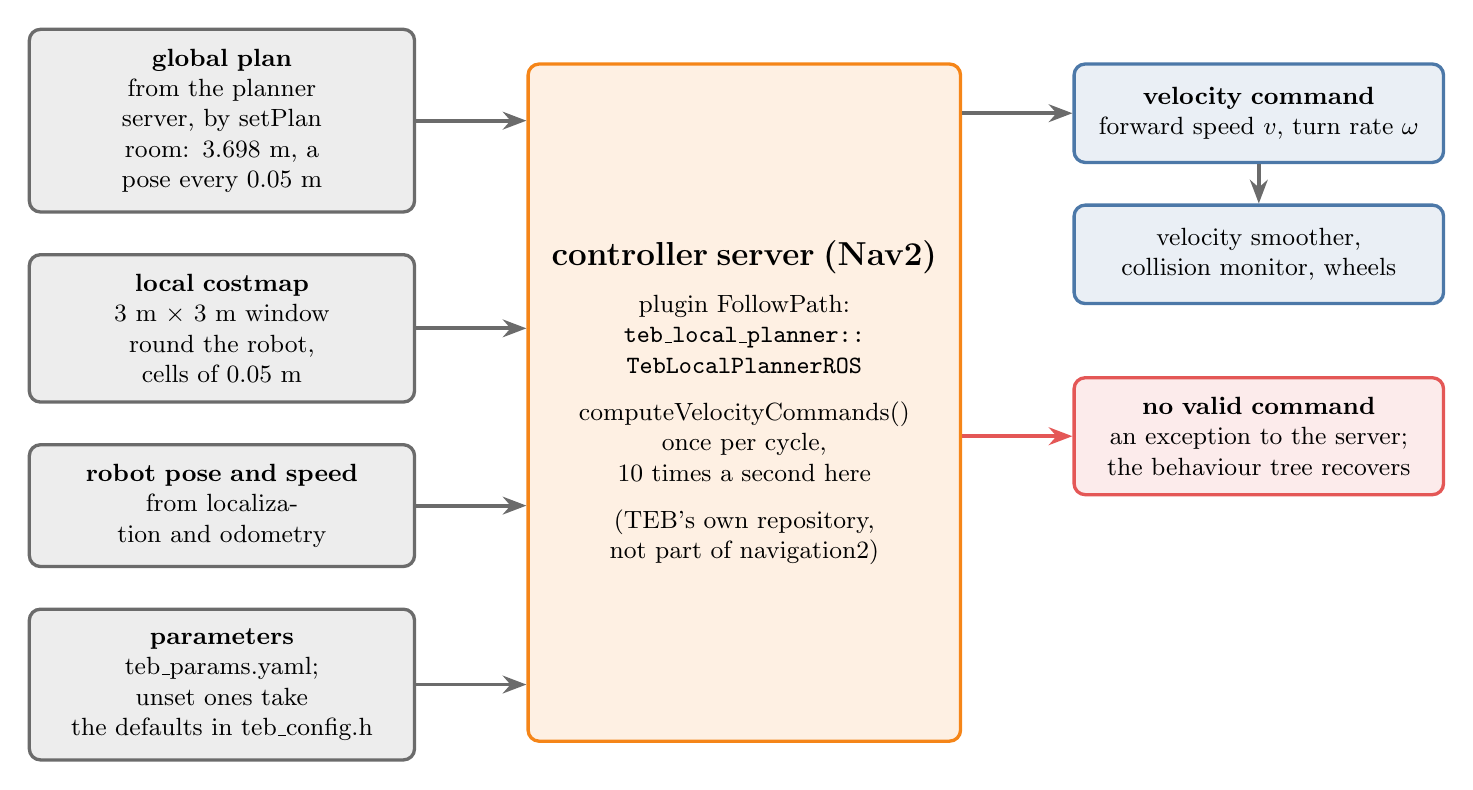
\begin{tikzpicture}[node distance=0.5cm,
  inp/.style={box=cgrey, font=\small, text width=4.4cm, minimum height=1.25cm},
  outb/.style={box=cblue, font=\small, text width=4.2cm, minimum height=1.25cm}]
  \node[inp] (plan) {\textbf{global plan}\\ from the planner server, by setPlan\\ room: 3.698 m, a pose every 0.05 m};
  \node[inp, below=of plan] (cm) {\textbf{local costmap}\\ 3 m $\times$ 3 m window round the robot,\\ cells of 0.05 m};
  \node[inp, below=of cm] (odo) {\textbf{robot pose and speed}\\ from localization and odometry};
  \node[inp, below=of odo] (par) {\textbf{parameters}\\ teb\_params.yaml; unset ones take\\ the defaults in teb\_config.h};
  \node[box=corange, font=\small, anchor=west,  text width=5.0cm, minimum height=8.6cm] (teb) at ($(plan.east)!0.5!(par.east) + (1.4,0)$)
    {\textbf{\large controller server (Nav2)}\\[6pt] plugin FollowPath:\\ \texttt{teb\_local\_planner::}\\ \texttt{TebLocalPlannerROS}\\[6pt]
     computeVelocityCommands()\\ once per cycle,\\ 10 times a second here\\[6pt] (TEB's own repository,\\ not part of navigation2)};
  \node[outb, right=1.4cm of teb.north east, anchor=north west] (cmd) {\textbf{velocity command}\\ forward speed $v$, turn rate $\omega$};
  \node[outb, below=of cmd] (base) {velocity smoother,\\ collision monitor, wheels};
  \node[box=cred, font=\small, text width=4.2cm, minimum height=1.25cm, below=0.9cm of base] (fail)
    {\textbf{no valid command}\\ an exception to the server;\\ the behaviour tree recovers};
  \foreach \n in {plan, cm, odo, par} \draw[arrow] (\n.east) -- (teb.west |- \n.east);
  \draw[arrow] (teb.east |- cmd.west) -- (cmd.west);
  \draw[arrow] (cmd) -- (base);
  \draw[arrow, draw=cred] (teb.east |- fail.west) -- (fail.west);
\end{tikzpicture}
\end{document}
